\chapter{State of the Art}


\begin{itemize}
    \item \enquote{Decentralized Deep Reinforcement Learning for a Distributed and Adaptive Locomotion Controller of a Hexapod Robot}
    \item Machine Learning in letzten Jahren erfolgreich auf viele Aufgaben angewandt
    \item DRL scheint noch Probleme zu haben bei der Anwendung für reale Roboter in \enquote{continuous control tasks}
    \item vor allem im Umgang mit unvorhergesehenen Situationen gibt es Probleme
    
    \item ursprünglich aus Bereich Computerspiele, deshalb viel in simulierten Umgebungen
    \item Transfer auf reale Probleme kann schwierig sein (\enquote{nature of such problems is fundamentally different from those in playing computer games})
    \item häufig wird zunächst die Simulation genutzt, um Grundsteine zu legen, die dann manuell feingeschliffen werden für eine bestimmte Aufgabe
    \item zwei fundamentale Probleme: soll den Reward ausnutzen, neigt deshalb zu Overfitting; reale Anwendungen deutlich mehr (Signal-)Rauschen, führt zu Hinterfragen von festem Markov Decision Process
    \item DRL tendiert dazu, Nischenlösungen zu finden, die meist nicht dazu in der Lage sind, adaptiv auf neue Situationen zu reagieren
    
    \item Tendenz geht dahin, hierarchische oder dezentralisierte Ansätze zu verfolgen
    \item hierarchisch erlaubt flexibles wechseln zwischen verschiedenen Unteraufgaben und Verhaltensweisen und somit auch Agieren in verschiedenen Kontexten möglich, bislang allerdings nur mit geringen Freiheitsgraden umgesetzt
    \item Fokus diesen Papers eher auf Störungen und Varietät in einem spezifischen Kontext mit einem spezifischen Verhalten
    
    \item PPO funktioniert allgemein gut mit kontinuierlichen Problemen ohne viel Hyperparameter-Tuning
    \item Median-Geschwindigkeit einer Episode ist der Reward
    \item \cite{schilling2020decentralized}
\end{itemize}

\begin{figure}
    \centering
    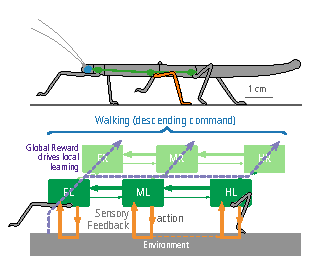
\includegraphics[width = 0.35\textwidth]{Bilder/decentralized-insect.pdf}
    \caption{\cite{schilling2020decentralized}}
\end{figure}


\hrule
\begin{itemize}
    \item \enquote{Adaptation of a Decentralized Controller to Curve Walking in a Hexapod Robot}
    \item bei Robotern mit mehreren Beinen aktuell drei vorherrschende Ansätze
    - Central Pattern Generators (CPGs)
        - Oszilatorsysteme oder neurale Netze, die rhythmische Ausgabe erzeugen, ohne bestimmte Eingabe vorauszusetzen
    - lernende Ansätze
    - Sensorenbasierte Ansätze
        - sind besser erklärbar verglichen mit lernenden Ansätzen
        - normalerweise relativ anpassbar an sich verändernde Umgebungen
    
    \item sehen Potenzial in Verbindung mehrerer Ansätze
    \item \cite{simmering2023walknet}
\end{itemize}


\hrule
\begin{itemize}
    \item \enquote{DeepGait: Planning and Control of Quadrupedal Gaits using Deep Reinforcement Learning}
    \item Kombination von state-of-the-art modellbasierten Methoden der Bewegungsplanung und Reinforcement Learning
    \item Evaluieren die physikalische Machbarkeit anstatt physisch zu simulieren
    \item trennen Schrittplanung und Ausführung
    \item es können ganze Schritte evaluiert werden und nicht nur einzelne Frames einer Simulation
    \item Hauptproblem in Schrittplanung ist Kombinatorik, wegen der vielen möglichen Kombinationsmöglichkeiten für Kontaktpunkte mit dem Untergrund
    \item aber: Training auf späterem Terrain, allerdings relativ gute Verallgemeinerung
    \item Entropie ist extrem wichtig
    \item Weit bessere Resultate als andere Ansätze, gerade was das Überbrücken von Klüften angeht
    \item \cite{tsounis2020deepgait}
\end{itemize}


\hrule
\begin{itemize}
    \item \enquote{Learning and Adapting Agile Locomotion Skills by Transferring Experience}
    \item selbst einfache Aufgaben können sehr komplexe modulierte Reward-Funktionen benötigen, um die gezielten Bewegungen zu erhalten
    \item Wenn eine Bewegungsform sehr gut koordinierte Bewegungen voraussetzt, kann sehr schwer sein, wenn man von Null beginnt (-> nur sehr konkretes Verhalten kann Reward nach sich ziehen)
    \item Für ein spezifisches Zielproblem zu trainieren mag schwer sein, doch häufig ist es möglich, mit einfacheren Trainingsumgebungen zumindest relevante Daten zu erhalten, welche für einen Lernprozess von Interesse sind
    \item (Aus auf Hinterbeinen stehen wird Laufen)
    \item Häufig ist es schwierig, das in agileres Verhalten zu erweitern; insbesondere mit stark angepassten Reward-Funktionen, um das Verhalten überhaupt erst zu erzeugen
    \item => Training Agiler Roboter Fähigkeiten erleichtern durch Transfer mit existierenden suboptimalen Fähigkeiten
    \item \cite{smith2023learning}
\end{itemize}

\begin{figure}
    \centering
    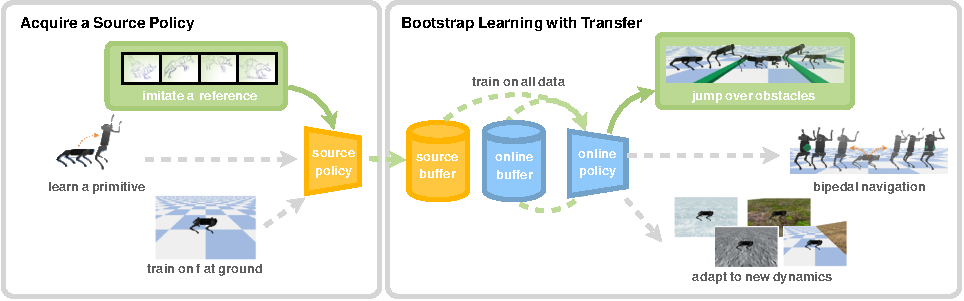
\includegraphics[width = \textwidth]{Bilder/transfer-learning.pdf}
    \caption{\cite{smith2023learning}}
\end{figure}